% compile with XeLaTeX or LuaLaTeX

\documentclass[12pt]{article}  % `article' with A4 paper size option

\usepackage{fontspec}
\setmainfont[
	Ligatures=TeX,
	Extension=.otf,
	SlantedFont=cmunsl,
	BoldFont=cmunbx,
	ItalicFont=cmunti,
	BoldItalicFont=cmunbi,
	SmallCapsFont=cmunrm, % for upright instead of slanted small caps
	SmallCapsFeatures={Letters=SmallCaps},	
]{cmunrm}

\usepackage{microtype}

\usepackage{polyglossia}
\setdefaultlanguage{spanish}
\setotherlanguage{russian}

\usepackage{amsmath,amssymb,color,amscd,wrapfig}
\usepackage{graphicx}

\marginparwidth 40pt
 \textwidth=140mm
 \textheight=206mm


\title{Problemas para j\`{o}venes de 5 a 15 a\~{n}os}

\author{V.\,I.~Arnold
\vspace*{2cm}\\ 
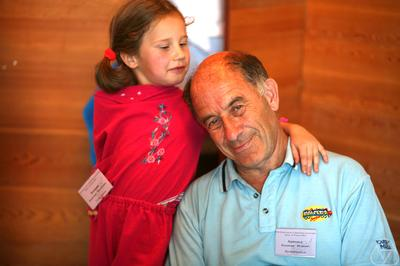
\includegraphics[width=12cm]{photo-arnold_small}
}

\date{}
\begin{document}
%\sloppy
\def\eps{\varepsilon}
%%\vskip7cm
\maketitle
\thispagestyle{empty}

\newpage 
\setcounter{page}{1}
\begin{abstract}

Este libro recoge una colecci\'on de 77 problemas, formulados o seleccionados por el propio autor, 
que favorecen el desarrollo del pensamiento.
La mayor\'{\i}a de ellos no requieren ning\'un conocimiento m\'as all\'a de una educaci\'on general, 
sin embargo, la resoluci\'on de algunos puede convertirse en un desaf\'{\i}o incluso para profesores 
universitarios.

El libro est\'a dirigido a estudiantes, desde el colegio hasta la universidad, a profesores, 
a padres y, en general, a todo el mundo que considere que el pensamiento es una parte fundamental del desarrollo personal.
\end{abstract}

\newpage


Reun\'{\i} estos problemas en unas hojas de papel en la primavera de 2004 en Par\'{\i}s, cuando unos rusos 
que viv\'{\i}an all\'{\i} me pidieron ayuda para que sus hijos adquirieran el pensamiento tradicional en Rusia.

Estoy profundamente convencido que esta cultura se basa principalmente en la reflexi\'on independiente y
temprana sobre lo simple, pero no sobre preguntas f\'aciles similares a las propuestas a continuaci\'on 
(los problemas 1, 3, 13 son los m\'as recomendados).

Mi larga experiencia ha mostrado que, con mucha frecuencia, los alumnos que suspenden en el colegio 
resuelven mejor los problemas que los mejores estudiantes de la clase, ya que -- para sobrevivir al final
 de la clase -- deben pensar permanentemente m\'as de lo necesario ``para ser los reyes de mambo", 
 como sol\'{\i}a decir F\'{\i}garo sobre s\'{\i} mismo,
cuando los estudiantes de sobresaliente no pueden entender qu\'e debe multiplicarse por qu\'e en estos problemas.
Tambi\'en he reparado en que los ni\~nos de cinco a\~nos resuelven problemas similares mejor 
que los alumnos que han sido contaminados al entrenarlos, que a su vez lo hacen mejor que universitarios, 
que ganan a sus profesores (los que peor han resuelto los problemas sencillos han sido los ganadores de los premios 
Nobel y Fields).   

\ 

\vspace{0pt plus 12pt}
\centerline{*\quad *\quad*}
\vspace{.4\baselineskip}

\

%\newpage
\noindent{\bf 1.} A Masha le faltan siete c\'opecas para comprar un libro de primera lectura, y a Misha le falta una.
Juntaron su dinero para comprar un solo libro y compartirlo, pero aun as\'{\i} no ten\'{\i}an suficiente.
?`Cu\'anto costaba el libro?
\newline\newline
{\bf 2.} Una botella con corcho cuesta 10 c\'opecas, y la botella en s\'{\i} es 9 c\'opecas m\'as cara 
que el corcho. ?`Cu\'anto cuesta la botella sin el corcho?
\newline\newline{}\quad
{\bf 3.} Un ladrillo pesa una libra y medio ladrillo. ?`Cu\'antas libras pesa el ladrillo?
\newline\newline\quad
{\bf 4.} Se toma una cucharada de vino de un barril y se vierte en una taza de t\'e (que no est\'a llena).
A continuaci\'on, con la misma cuchara, se toma una cucharada de esta mezcla (no homog\'enea) de la taza y se vuelve a 
poner en el barril.
Ahora tanto el barril como la taza tienen un cierto volumen de un l\'{\i}quido extra\~no (vino en la taza y t\'e en el
 barril). ?`En cu\'al de ellos el volumen del l\'{\i}quido extra\~no es mayor: en la taza o en el barril?
\newline\newline\quad
{\bf 5.} Dos viejecitas partieron respectivamente desde $A$ hacia $B$ y desde $B$ hacia $A$ al amanecer dirigi\'endose la
 una hacia la otra (por la misma carretera). Se encontraron al mediod\'{\i}a pero no pararon, y cada una continu\'o su 
 camino a la misma velocidad. La primera se\~nora lleg\'o (a $B$) a las 4pm, y la segunda (a $A$) a las 9pm. ?`A qu\'e
  hora amaneci\'o aquel d\'{\i}a? 
\newline\newline\quad
{\bf 6.} La hipotenusa de un tri\'angulo rect\'angulo (en un examen est\'andar americano) mide 10 pulgadas,
la altura proyectada sobre ella mide 6 pulgadas. Calcular el \'area del tri\'angulo.
%\newline

Los estudiantes americanos se hab\'{\i}an enfrentado a este problema durante d\'ecadas, pero llegaron estudiantes rusos,
 de Mosc\'u, y ninguno de ellos fue capaz de encontrar la respuesta como lo hac\'{\i}an sus compa\~neros americanos 
 (dando como respuesta 30 pulgadas). ?`Por qu\'e?
\newline\newline\quad
{\bf 7.} Vasya tiene 2 hermanas m\'as que hermanos. ?`Cu\'antas hijas m\'as que hijos tienen sus padres?
\newline\newline\quad
{\bf 8.} Hay un lago redondo en Am\'erica del Sur. Cada a\~no, el 1 de junio, aparece en el centro una flor Victoria Regia
 (el tallo emerge desde el fondo, y sus p\'etalos est\'an sobre el agua como los de un nen\'ufar). Cada d\'{\i}a se dobla
  el \'area de la flor, y el 1 de julio, la flor cubre por fin todo el lago, pierde los p\'etalos, y la semilla se hunde
   en el fondo. ?`En qu\'e fecha el \'area de la flor es la mitad del \'area del lago?    
\newline\newline\quad
{\bf 9.} Un campesino tiene que transportar un lobo, una cabra y un repollo de una orilla a otra del r\'{\i}o en una barca.
 Sin embargo la barca es tan peque\~na que s\'olo hay sitio para \'el y uno de los tres. ?`C\'omo deber\'{\i}a
  transportarlos a los tres de una orilla a otra? (El lobo y la cabra no pueden quedarse solos, y la cabra y el repollo
   tampoco)
\newline\newline\quad
{\bf 10.} Durante el d\'{\i}a un caracol sube 3 cent\'{\i}metros en un poste, y durante la noche, como se duerme, resbala
 accidentalmente 2 cm hacia abajo. El poste tiene 10 m de altura, y encima de \'el hay un manjar (para el caracol). 
  ?`Cu\'anto tiempo tardar\'a en alcanzar el manjar?
\newline\newline\quad
{\bf 11.} Un guardabosques camina desde su tienda 10 km en direcci\'on sur, gira hacia el este, camina en l\'{\i}nea recta
 10 km m\'as en direcci\'on este, se encuentra con su amigo el oso, gira hacia el norte , y despu\'es de 10 km vuelve a
  estar en la tienda. ?`De qu\'e color era el oso y d\'onde ocurri\'o todo esto?
\newline\newline\quad
{\bf 12.} Hoy a las 12 del mediod\'{\i}a hubo pleamar. ?`A qu\'e hora ser\'a la pleamar en el mismo sitio (en el mismo lugar)
 ma\~nana?
\newline\newline\quad
{\bf 13.} Los dos primeros vol\'umenes de Pushkin est\'an uno al lado del otro en una estanter\'{\i}a. 
Las p\'aginas de cada uno de ellos tienen un grosor de 2 cm, y las cubiertas --delantera y trasera 
-- de 2 mm. Una polilla ha carcomido el libro (perpendicularmente a las p\'aginas) desde la primera del volumen 1 hasta
 la \'ultima del volumen 2.
%\begin{wrapfigure}{r}{3cm}
%\vspace{-\baselineskip}
%\centering % \advance\rightskip2.5mm 
%\footnotesize
%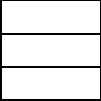
\includegraphics{taskbook-99}\\[2pt]
%Top view\\[6pt]
%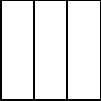
\includegraphics{taskbook-98}\\[2pt]
%Front view\\[24pt]
%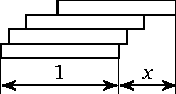
\includegraphics{taskbook-97}\\[24pt]
%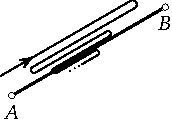
\includegraphics{taskbook-1}\\[18pt]
%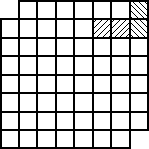
\includegraphics{taskbook-2}\\[6pt]
%\end{wrapfigure}
?`Cu\'anto mide el rastro que ha dejado la polilla?
%\newline

[Este problema topol\'ogico con una respuesta incre\'{\i}ble -- 4 mm -- es imposible para los acad\'emicos,
 pero hay ni\~nos peque\~nos que lo resuelven f\'acilmente.]  
\newline\newline\quad
{\bf 14.} Encontrar el cuerpo cuyas vistas en planta y alzado sean como las que se representan (politopos).
Representar su perfil (dibujando los lados invisibles del politopo en l\'{\i}nea discont\'{\i}nua).
\begin{figure}[h]
\centering
\footnotesize
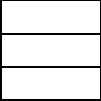
\includegraphics[scale=1]{taskbook-99} \qquad\qquad
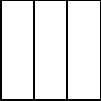
\includegraphics[scale=1]{taskbook-98}
\\[2pt]
\hspace{1pt} 
Planta
\hspace{43pt} Alzado
\end{figure}
\newline\quad
{\bf 15.} ?`De cu\'antas maneras se puede descomponer el n\'umero 64 en 10 sumandos naturales (enteros $\ge 1$),
tales que el m\'aximo sea 12?
%\newline
[Las formas que s\'olo difieran en el orden de los sumandos no se cuentan como diferentes.]
\newline\newline\quad
{\bf 16.} Colocando unas cuantas barras una sobre otra (por ejemplo, piezas de domin\'o),
se puede conseguir una longitud $x$ de la parte que cuelga. ?`Cu\'al es el m\'aximo valor esperado para la longiud 
 $x$ de la parte que cuelga?

\begin{figure}[h!]
\centering
\footnotesize
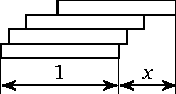
\includegraphics[scale=1]{taskbook-97}
\end{figure}
%\newline\newline\quad
\begin{figure}[h]
\begin{minipage}[c][][c]{0.7 \textwidth}

\newpage
{\bf 17.} La distancia entre las ciudades $A$ y $B$ es de 40 km. Dos ciclistas salen respectivamente de $A$ y de $B$ 
a la vez, dirigi\'endose el uno hacia el otro, uno con velocidad de 10 km/h y el otro con velocidad de 15 km/h. 
Una mosca sale desde el primer ciclista cuando est\'a en $A$ volando a una velocidad de 100km/h, toca la frente del 
segundo, vuelve a volar hasta la frente del primero, regresa hasta la del segundo, y contin\'ua as\'{\i} hasta que las 
frentes de los ciclistas se chocan y aplastan a la mosca.
?`Cu\'antos kil\'ometros ha volado en total la mosca?
\end{minipage}
\hfill
\begin{minipage}[c]{0.2 \textwidth}
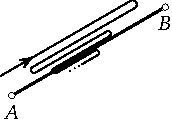
\includegraphics[scale=1]{taskbook-1}
\end{minipage}
\end{figure}

%\newline\newline\newline\quad

%{\bf 17.} The distance between cities $A$ and $B$ is 40 km. Two cyclists leave respectively from $A$ and $B$ simultaneously
%towards one another, one with speed 10 km/h and the other with speed 15 km/h. A fly flies out with the first
%cyclist from $A$ with the speed of 100km/h, reaches the second, touches his forehead and flies back to the first,
%touches his forehead, returnes to the second, and so on until the cyclists' foreheads collide and squash
%the fly.
%How many kilometers altogether has the fly flown?
%\begin{figure}[h]
%\centering
%\footnotesize
%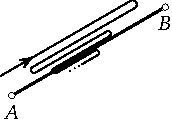
\includegraphics[scale=1]{taskbook-1}
%\end{figure}
\medskip\noindent
{\bf 18.} Una pieza de domin\'o cubre dos casillas de un tablero de ajedrez. 
Cubrir todos los cuadrados excepto los dos opuestos (en la misma diagonal) con 31 piezas. [Un tablero de ajedrez est\'a formado por $8 \times 8 = 64$ casillas.]
\begin{figure}[h]
\centering
\footnotesize
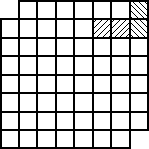
\includegraphics[scale=1]{taskbook-2}
\end{figure}
%\newline\quad

%newpage
\noindent{\bf 19.} Una oruga quiere deslizarse desde una esquina de una habitaci\'on c\'ubica (la esquina izquierda del suelo) a la opuesta (la esquina derecha del techo).
%\begin{wrapfigure}{r}{3.0cm}
%\centering 
%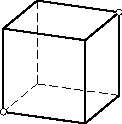
\includegraphics{taskbook-3}\\[8pt]
%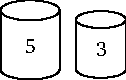
\includegraphics{taskbook-4}\\[8pt]
%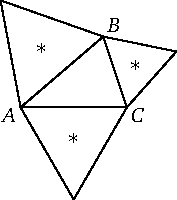
\includegraphics{taskbook-6}\\[8pt]
%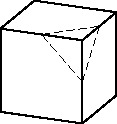
\includegraphics{taskbook-7}\\[8pt]
%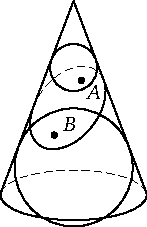
\includegraphics{taskbook-9}\\[6pt]
%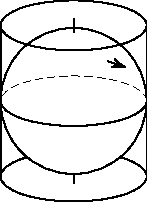
\includegraphics{taskbook-10}\\[6pt]
%\end{wrapfigure}
Encontrar el camino m\'as corto para el viaje por las paredes de la habitaci\'on.
\begin{figure}[h]
\centering
\footnotesize
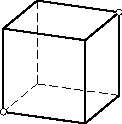
\includegraphics[scale=1]{taskbook-3}
\end{figure}
\newline\newline\quad
{\bf 20.} Se tienen dos vasos de vol\'umenes 5 litros y 3 litros. Medir un litro (obtenerlo en uno de los vasos).

\begin{figure}[h!]
\centering
\footnotesize
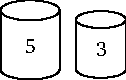
\includegraphics[scale=1]{taskbook-4}
\end{figure}

%\newline\newline\quad
\medskip\noindent
{\bf 21.} En una familia hay cinco cabezas y catorce piernas. ?`Cu\'antas personas y cu\'antos perros forman la familia?
%\newline\quad
\begin{figure}[h!]
\begin{minipage}[c][][c]{0.7 \textwidth}
{\bf 22.} En cada uno de los lados $AB$, $BC$ y $CA$ del tri\'angulo $ABC$ se construye hacia fuera un tri\'angulo equil\'atero.
Probar que sus centros ($*$) forman un tri\'angulo equil\'atero.\end{minipage}
\hfill
\begin{minipage}[c]{0.2 \textwidth}
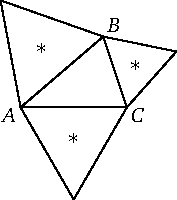
\includegraphics[scale=1]{taskbook-6}
\end{minipage}
\end{figure}

%{\bf 22.} Equilateral triangles are constructed externally on sides $AB$, $BC$ and $CA$ of a triangle $ABC$.
%Prove that their centres ($*$) form an equilateral triangle.
%\begin{figure}[h]
%\centering
%\footnotesize
%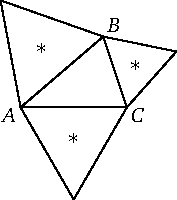
\includegraphics[scale=1]{taskbook-6}
%\end{figure}

\newpage
\noindent
{\bf 23.} ?`Qu\'e pol\'{\i}gonos se pueden obtener al intersecar un cubo con un plano? ?`Se puede obtener un pent\'agono? ?`Un hept\'agono? 
?`Un hex\'agono regular?
\begin{figure}[h]
\centering
\footnotesize
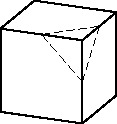
\includegraphics[scale=1]{taskbook-7}
\end{figure}
\newline\newline\quad
{\bf 24.} Dibujar una recta que pase por el centro de un cubo y tal que la suma de los cuadrados de las distancias a los ocho v\'ertices del cubo sea:
a) m\'axima,
\newline
b) m\'{\i}nima (comparar con otras rectas que pasen por el centro).
\newline\newline\quad
{\bf 25.} Un cono circular recto se corta con un plano dando lugar a una curva cerrada. Se inscriben dos bolas en el cono, tangentes al plano en los puntos $A$ y $B$ respectivamente. 
Encontrar un punto $C$ en la l\'{\i}nea de corte tal que la suma de las distancias $CA + CB$ sea:
 a) m\'axima, b) m\'{\i}nima.
\begin{figure}[h]
\centering
\footnotesize
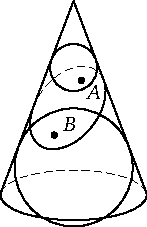
\includegraphics[scale=1]{taskbook-9}
\end{figure}
\newline\newline\quad
{\bf 26.} La superficie de la Tierra se proyecta sobre un cilindro formado por rectas tangentes a los meridianos en el Ecuador siguiendo rayos paralelos al Ecuador y que pasan por el eje que une los polos.
?`El \'area de la proyecci\'on de Francia ser\'a mayor o menor que el \'area de la propia Francia?
\begin{figure}[h]
\centering
\footnotesize
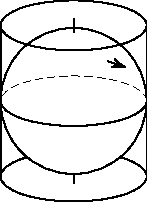
\includegraphics[scale=1]{taskbook-10}
\end{figure}

\newpage
\noindent
{\bf 27.} Probar que al dividir el n\'umero $2^{p-1}$ por el primo impar $p$ es resto es 1
(ejemplos: $2^2 = 3a +1,$ $2^4 = 5b+1,$ $2^6 = 7c+1,$ 
%\begin{wrapfigure}{r}{3cm}
%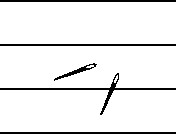
\includegraphics{taskbook-12}\\[12pt]
%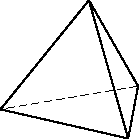
\includegraphics{taskbook-131}\\tetrahedron (tetra${}= 4$)\\[8pt]
%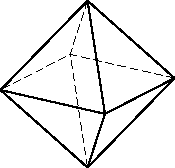
\includegraphics{taskbook-132}\\octahedron (octo${}= 8$)\\[8pt]
%{\Huge {}\hskip20pt ?}\\ icosahedron\vspace{3pt}
%\end{wrapfigure}
$2^{10} - 1 = 1023 = 11\cdot 93$).  
\newline\newline\quad
{\bf 28.} Una aguja de 10 cm de longitud se lanza aleatoriamente sobre un papel de rayas con un espaciado de 10 cm entre dos rayas consecutivas. 
Se repite esto $N$ (un mill\'on) veces. 
?`Cu\'antas veces (aproximadamente, salvo un peque\~no error en el porcentaje) la aguja intersecar\'a alguna raya del papel?
\begin{figure}[h]
\centering
\footnotesize
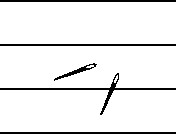
\includegraphics[scale=1]{taskbook-12}
\end{figure}
%\newline\quad

Uno puede realizar este experimento (como lo hice yo cuando ten\'{i}a 10 a\~nos) con $N=100$ en lugar de un mill\'on de lanzamientos.
[La respuesta a este problema es sorprendente: $\frac2{\pi}N$. Adem\'as incluso doblando la aguja hasta una longitud $a \cdot 10$
cm el n\'umero de intersecciones observadas en $N$ lanzamientos es aproximadamente $\frac{2a}{\pi}N$. 
El n\'umero $\pi \approx  \frac{355}{113} \approx \frac{22}7.$]
\newline\newline\quad
{\bf 29.} Los poliedros con caras triangulares son, por ejemplo, s\'olidos plat\'onicos: tetraedro (4 caras), octaedro (8 caras), icosaedro (20 -- y todas las caras son iguales; es interesante dibujarlo, tiene 20 v\'ertices y 30 aristas).
\begin{figure}[h!]
\centering
\footnotesize
\hspace{5pt}
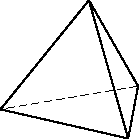
\includegraphics[scale=1]{taskbook-131}\hspace{68pt}
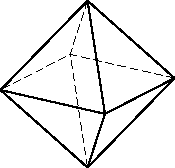
\includegraphics[scale=1]{taskbook-132}\\ \vspace{3pt}
tetraedro (tetra${}= 4$) \hspace{40pt}
octaedro (octo${}= 8$)\\[25pt]
{\Huge 
%{}\hskip20pt 
?}\\ icosaedro\vspace{3pt}
\end{figure}
\newline\quad

?`Es cierto que para todos \'estos (poliedros cerrados convexos con caras triangulares) el n\'umero de caras es igual a dos veces el n\'umero de v\'ertices menos cuatro?

\newpage
\noindent
%\newline\newline\quad
{\bf Otro s\'olido plat\'onico (en total hay 5):}
\begin{figure}[h]
\centering
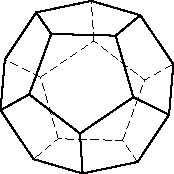
\includegraphics{taskbook-14}\\[2pt]
\end{figure}

\noindent
{\bf 30.} Un dodecaedro es un poliedro convexo con doce caras que son pent\'agonos (regulares), veinte v\'ertices y treinta aristas
 (sus v\'ertices son los centros de las caras de un icosaedro).

Inscribir en un dodecaedro cinco cubos (los v\'ertices de cada cubo son v\'ertices del dodecaedro)
cuyas aristas son diagonales de las caras del dodecaedro (el dodecaedro tiene 12 aristas, una en cada cara).
[Esto lo invent\'o Kepler al interesarse por los planetas.] 

\bigskip
\noindent{\bf 31.} Encontrar la intersecci\'on de dos tetraedros inscritos en un cubo (tales que los v\'ertices de cada uno lo son tambi\'en del cubo, y las aristas son diagonales de las caras). 

?`Qu\'e fracci\'on del volumen del cubo est\'a contenido en la intersecci\'on de los tetraedros?
\newline\newline\quad
$\mathbf 31^{bis}.$ Construir la secci\'on de un cubo por un plano que pasa por tres puntos dados en las aristas.
[Dibujar el pol\'{\i}gono resultante de la intersecci\'on con las caras del cubo.]
\begin{figure}[h]
\centering
% 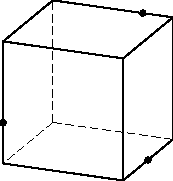
\includegraphics{taskbook-15}
\end{figure}

\noindent{\bf 32.} ?`Cu\'antas simetr\'{\i}as tiene tetraedro??`Cu\'antas tiene un cubo??`Y un octaedro??`Y un icosaedro? ?`Y un dodecaedro? La simetr\'{\i}a es una transformaci\'on que conserva las distancias.

Entre las simetr\'{\i}as, ?`cu\'antas rotaciones hay? y entre \'estas, ?`cu\'antas reflexiones? (en cada uno de los cinco casos propuestos)

\newpage
\noindent{\bf 33.} ?`De cu\'antas formas diferentes se pueden colorear las 6 caras un cubo con seis colores (1,...,6) [uno por cada cara]
de modo que los las formas sean distintos dos a dos (es decir, no se puede pasar de una forma a otra mediante una rotaci\'on)? 
\begin{figure}[h]
\centering
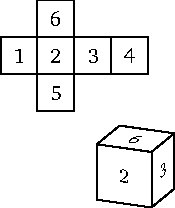
\includegraphics{taskbook-17}
\end{figure}


\noindent{\bf 34.} ?`De cu\'antas formas distintas se pueden permutar $n$ objetos?

Hay seis permutaciones posibles para $n=3$: (1,2,3), (1,3,2), (2,1,3), (2,3,1), (3,1,2), (3,2,1). ?`Cu\'antas hay para: $n=4$? $n=5$? $n=6$? $n=10$?
\begin{figure}[h]
\centering
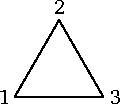
\includegraphics{taskbook-18}
\end{figure}

\noindent{\bf 35.} Un cubo tiene 4 diagonales largas ?`Cu\'antas permutaciones distintas de estos cuatro objetos se obtienen por rotaci\'on del cubo?
\begin{figure}[h]
\centering
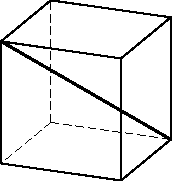
\includegraphics{taskbook-19}
\end{figure}

\noindent{\bf 36.} La suma de los cubos de tres enteros se resta del cubo de la suma de estos n\'umeros. ?`Esta diferencia es siempre divisible por 3?

\bigskip
\noindent{\bf 37.} Misma pregunta con la potencia quinta y la divisivilidad por 5, y para la potencia s\'eptima y la divisibilidad por 7.

\bigskip
\noindent{\bf 38.} Calcular la siguiente suma (con un margen de error del $1\%$).
$${1 \over 1\cdot 2} +  {1 \over 2\cdot 3} + {1 \over 3\cdot 4} + \dots + {1 \over 99\cdot 100}$$


\bigskip
\noindent{\bf 39.} Si dos pol\'{\i}gonos tienen el mismo area, entonces se pueden cortar en un n\'umero finito de pol\'{\i}gonos, que reordenados permiten obtener el segundo a partir del primero y viceversa. !`Probarlo! [Para s\'olidos en el espacio esto no ocurre: !`un cubo y un tetraedro con el mismo volumen no se pueden cortar de esta forma!]
\begin{figure}[h]
\centering
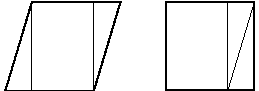
\includegraphics{q39_horizontal}\\[6pt]
\end{figure}


\noindent{\bf 40.} Se eligen 4 v\'ertices de un paralelogramo entre los nodos de una cuadr\'{\i}cula. Si ning\'un nodo de la cuadr\'{\i}cula queda encerrado en el interior del paralelogramo, probar que el \'area del paralelogramo es igual al de cada uno de los cuadros de la cuadr\'{\i}cula. 
\begin{figure}[h]
 \centering
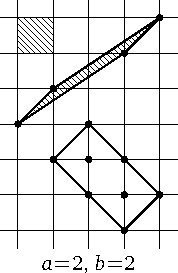
\includegraphics{taskbook-24}\vskip3pt
\end{figure}

\medskip
\noindent{\bf 41.} Con las condiciones de la pregunta 40, si $a$ nodos est\'an encerrados en el interior del paralelogramo y $b$ nodos est\'an en la frontera. Calcular el \'area del paralelogramo. 

\bigskip
\noindent{\bf 42.} Para paralelep\'{\i}pedos en tres dimensiones, ?`sigue siendo cierta la afirmaci\'on de la pregunta 40?

\bigskip
\noindent{\bf 43.} Los n\'umeros del conejo (o de Fibonacci) forman la secuencia $(a_1=1)$, $1$, $2$, $3$, $5$, $8$, $13$, $21$,
$34$,\nobreak\ $\dots$, en la que $a_{n+2}=a_{n+1}+a_n$ para cada
$n=1$, $2$,\nobreak\ $\dots$ \   Encontrar el m\'aximo com\'un divisor (mcd) de los n\'umeros $a_{100}$ y $a_{99}$.

\newpage
%\bigskip

\noindent{\bf 44.} Encontrar el n\'umero (de Catalan) de formas de dividir un $n$-\'agono convexo en tri\'angulos cort\'andolo por las diagonales que no se intersequen. 
Por ejemplo, $c(4)=2$, $c(5)=5$, $c(6)=14$. ?`Cu\'antos se pueden encontrar para $c(10)$?
\begin{figure}[h]
\centering
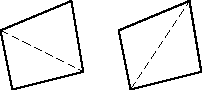
\includegraphics[scale=1]{taskbook-281}
\hskip1cm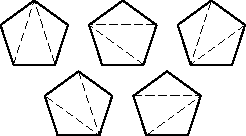
\includegraphics[scale=1]{taskbook-282}
\end{figure}


%\newpage
\bigskip
\noindent{\bf 45.} En un torneo participan $n$ equipos, los que pierden abandonan la competici\'on, y el ganador se decide tras $n-1$ encuentros.
El cuadro del torneo se puede escribir de forma simb\'olica como, por ejemplo,  $((a,(b,c)),d)$ que significa que $b$ juega contra $c$, y el ganador se cruza con $a$, y el ganador de \'estos con $d$].

?`Cu\'antos cuadros distintos hay para 10 equipos? 

Para 2 equipos, s\'olo puede ser $(a,b)$, luego un solo cuadro.

%{\advance\thinmuskip-2mu
%\noindent 
Para 3 equipos, s\'olo puede ser $((a,b),c)$, o $((a,c),b)$, o $((b,c),a)$, luego hay 3 posibles cuadros.

%\noindent 
Para 4 equipos:
%{\allowdisplaybreaks \advance\thinmuskip-.55mu
$$\begin{array}{cccc}
(((a,b),c),d) & \quad (((a,c),b),d) & \quad (((a,d),b),c) & \quad (((b,c),a),d) \\
(((b,d),a),c) & \quad (((c,d),a),b) & \quad (((a,b),d),c) & \quad (((a,c),d),b) \\ 
(((a,d),c),b) & \quad (((b,c),d),a) & \quad (((b,d),c),a) & \quad (((c,d),b),a) \\
((a,b),(c,d)) & \quad ((a,c),(b,d)) & \quad ((a,d),(b,c))
% \displaybreak[4]
\end{array}$$

\bigskip
\noindent{\bf 46.} Unir $n$ puntos $1, 2, \dots, n$ con $n-1$ trazos (en una sola pieza) para obtener un \'arbol. ?`Cu\'antos \'arboles distintos se pueden obtener (!`el caso $n=5$ ya es interesante!)?
 
\medskip
%$n=2$:\quad 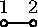
\includegraphics{taskbook-291}\,,\quad el n\'umero es 1; 

\medskip
$n=3$:\quad 
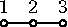
\includegraphics{taskbook-292}\,,\quad 
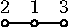
\includegraphics{taskbook-293}\,,\quad 
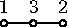
\includegraphics{taskbook-294}\,,\quad 
el n\'umero es 3;

\medskip
$n=4$:\quad\def\quad{\hskip.7em}
$\vcenter{\hbox{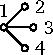
\includegraphics{taskbook-295}}}$,\quad
$\vcenter{\hbox{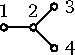
\includegraphics{taskbook-296}}}$,\quad
$\vcenter{\hbox{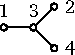
\includegraphics{taskbook-297}}}$,\quad
$\vcenter{\hbox{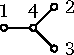
\includegraphics{taskbook-298}}}$,\quad
$\vcenter{\hbox{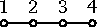
\includegraphics{taskbook-299}}\hbox{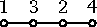
\includegraphics{taskbook-290}}
\vskip-8pt
\hbox to50bp{\dotfill}}$,\quad 
el n\'umero es 16.


\newpage
%\bigskip
\noindent{\bf 47.} Una pernutaci\'on $(x_1,x_2, \dots,x_n)$ de los n\'umeros $\{1, 2, \dots, n\}$ se denomina una
    \emph{serpiente} (de longitud $n$) si $x_1<x_2>x_3<x_4 \dots$ \  .
    \medskip

%\noindent
{\sc Ejemplo:}
$\begin{aligned}[t]
&\begin{aligned}[t] n=2, \text{ only }  1<2, \end{aligned} &&\text{el n\'umero es  }1, \\
&\hskip-\nulldelimiterspace\mathord{\left.\begin{aligned} n=3, \hphantom{\text{ only }} 1&<3>2 \\ 
                                              2&<3>1\end{aligned} \right\}}, && \text{el n\'umero es  }2,  \\[2pt]
&\hskip-\nulldelimiterspace\mathord{\left.\begin{aligned} n=4, \hphantom{\text{ only }} 1&<3>2<4 \\ 
                                              1&<4>2<3 \\ 
                                    2&<3>1<4 \\ 
                                    2&<4>1<3 \\ 
                                    3&<4>1<2\end{aligned} \right\}},
                                    &&\text{el n\'umero es  }5. \\
\end{aligned}$

%\vspace{\jot}
%$$\begin{aligned}[h]
%&\begin{aligned}[h] n=2, {\rm only }  1<2, \end{aligned} &&{\rm the \  number}=1, \\
%&\hskip-\nulldelimiterspace\mathord{\left.\begin{aligned} n=3, \hphantom{{\rm only}} 1&<3>2 \\ 
%                                              2&<3>1\end{aligned} \right\}}, && {\rm the \  number}=2,  \\[2pt]
%&\hskip-\nulldelimiterspace\mathord{\left.\begin{aligned} n=4, \hphantom{{\rm only }} 1&<3>2<4 \\ 
%                                              1&<4>2<3 \\ 
%                                    2&<3>1<4 \\ 
%                                    2&<4>1<3 \\ 
%                                    3&<4>1<2\end{aligned} \right\}},
%                                    &&{\rm the \  number}=5. \\
%\end{aligned}$$

%\vspace{\jot}
\medskip
\noindent 
Encontrar el n\'umero de serpientes de longitud 10.

%\newpage
\bigskip
\noindent{\bf 48.} Sea $s_n$ el n\'umero de serpientes de longitud $n$:
$$
s_1=1, \quad s_2=1, \quad s_3=2, \quad s_4=5, \quad s_5=16, \quad s_6=61.
$$
Probar que la serie de Taylor de la tangente es:
$$
\tan x=1\, \frac{x^1}{1!}+2\, \frac{x^3}{3!}+16\, \frac{x^5}{5!}+\dots=
\textstyle\sum\limits_{k=1}^{\infty} s_{2k-1}\, \frac{x^{2k-1}}{(2k-1)!}.
$$
 

\bigskip
\noindent{\bf 49.} Encontrar la suma de las series
$$
1+1\, \frac{x^2}{2!}+5\, \frac{x^4}{4!}+61\, \frac{x^6}{6!}+\dots=
\textstyle\sum\limits_{k=0}^{\infty} s_{2k}\,\frac{x^{2k}}{(2k)!}.
$$

\bigskip
\noindent{\bf 50.} Para $s>1$, probar la identidad
$$
\textstyle\prod\limits_{p=2}^{\infty} \cfrac{1}{1-\cfrac{1}{p^s}}=\sum\limits_{n=1}^{\infty} \frac{1}{n^s}
$$ 
(el producto afecta a todos los n\'umeros primos $p$, y el sumatorio a los n\'umeros naturales ~$n$).

%\newpage
\bigskip
\noindent{\bf 51.} Encontrar la suma de las series
$$
1+ \frac{1}{4}+ \frac{1}{9}+\dots=\textstyle\sum\limits_{n=1}^{\infty} \frac{1}{n^2}
$$
(probar que es $\pi^2/6$, es decir, aproximadamente $3/2$). 

\newpage
%\bigskip
\noindent{\bf 52.} Encontrar la probabilidad de una fracci\'on $p/q$ sea irreducible (se define de la siguiente forma:
en el disco $p^2+q^2 \leqslant R^2$, se cuenta el n\'umero $N$ de vectores con dos componentes enteras $p$ y $q$ que no tengan divisores comunes mayores que 1, despu\'es de hacer \'esto, la probabilidad de que sea irreducible es el l\'{\i}mite del cociente $N(R)/M(R)$, donde $M(R)$ es el n\'umero de puntos enteros en el disco $(M \sim \pi R^2)$).
\begin{figure}[h]
\footnotesize
\centering
\includegraphics{taskbook-36}\\{\ } \\
$M(5)=81$, $N(5)=44$, $N/M = 44/81$
\end{figure}

\bigskip
\noindent{\bf 53.} Para la secuencia de los n\'umeros de Fibonacci $a_n$ del problema 43, encontrar el l\'{\i}mite del cociente 
$a_{n+1}/a_n$ cuando $n$ tiende a infinito:\vspace{2\jot}
\[
\frac{a_{n+1}}{a_n}=2,\ \frac 32,\ \frac53, \ \frac85, \ \frac{13}8,
\ \frac{34}{21}.
\vspace{\jot}
\] 

%\noindent
\textsc{Respuesta:} ``la raz\'on aurea o n\'umero aureo",
$\frac{\sqrt{5}+1}{2\vphantom)} \approx 1{,}618$. [Es la raz\'on de los lados de una tarjeta que es similar a la tarjeta resultante de quitar el cuadrado de lado el menor lado de la tarjeta,
  $\frac{AB}{BC}=\frac{PC}{CD\vphantom)}$.] ?`Cu\'anto vale la raz\'on aurea relativa a un pent\'agono regular y una estrella de 5 puntas? 

\begin{figure}[h]
\centering
\includegraphics{taskbook-37}
\end{figure}

\newpage
%\medskip
\noindent{\bf 54.} Calcular la fracci\'on cont\'{\i}nua infinita
\begin{align*}
1+\cfrac{1}{2+\cfrac{1}{1+\cfrac{1}{2+\cfrac{1}{1+\cfrac{1}{2+\ldots}}}}}=
a_0+\cfrac{1}{a_1+\cfrac{1}{a_2+\cfrac{1}{a_3+\dots}}} \qquad
\smash{
%\medmath
{\left[\begin{aligned} &a_{2k}=1 \\[-\jot] &a_{2k+1}
      =2 \end{aligned}\right]} }
\end{align*}

\medskip

\noindent (es decir, el l\'{\i}mite de las fracciones
$$
a_0+\cfrac{1}{a_1+\cfrac{1}{a_2+{\atop{\ddots \atop {}} + \cfrac{1}{a_n}}
} 
}
$$
cuando $n \to \infty$).


\bigskip
\noindent{\bf 55.} Encontrar los polinomios
\[
y=\cos 3 (\arccos x),\  y=\cos 4 (\arccos x),\ 
y=\cos n (\arccos x),
\] 
para $|x| \leqslant 1$. 


\bigskip
\noindent{\bf 56.} Calcular la suma de las potencias $k$-\'esimas para los $n$ complejos ra\'{\i}ces $n$-\'esimas de la unidad.  
 

\bigskip
\noindent{\bf 57.} En el plano $(x,y)$, dibujar las curvas definidas param\'etricamente por: 
\[
\{x=\cos 2t, y=\sin 3t\},\quad 
\{x=t^3-3t, y=t^4-2t^2\}.
\]

\bigskip
\noindent{\bf 58.} Calcular (con una cota de error menor del 10\%)
$$
\int\limits_0^{2\pi} \sin^{100} x\,dx.
$$

\bigskip
\noindent{\bf 59.} Calcular (con una cota de error menor del 10\%)
$$
\int\limits_1^{10} x^x\,dx.
$$

\bigskip
\noindent{\bf 60.} Encontrar el \'area de un tri\'angulo cuyos \'angulos $(\alpha, \beta, \gamma)$ est\'an en una esfera de radio 1,
y cuyos lados son circunferencias grandes (secciones de una esfera con un plano que pasa por el centro de la esfera).

\medskip
%\noindent
\textsc{Respuesta:} $S=\alpha+\beta+\gamma-\pi$ (por ejemplo, en un tri\'angulo con tres \'angulos rectos, $S=\pi/2$, es decir, la octava parte del \'area total de la esfera).
\begin{figure}[h]
\centering
 \includegraphics{taskbook-44}\hskip2cm \includegraphics{taskbook-45}
\end{figure}

\bigskip
\noindent{\bf 61.} Un c\'{\i}rculo de radio $r$ rueda (sin deslizarse) por el interior de un c\'{\i}rculo de radio 1.
Dibujar la trayectoria completa de un punto del c\'{\i}rculo que se desplaza (esta trayectoria se denomina hipocicloide) 
para $r=1/3$, para $r=1/4$, para $r=1/n$, y para $r=1/2$.

\bigskip
\noindent{\bf 62.} En una clase de $n$ alumnos, estimar la probabilidad de haya dos que cumplan a\~nos el mismo d\'{\i}a. ?`Es alta o baja?

%\noindent
\medskip
\textsc{Respuesta:} (muy) alta si el n\'umero de alumnos es (bastante) mayor que $n_0$,
(muy) baja si es (bastante) m\'as peque\~no que $n_0$, y hay que buscar qu\'e es realmente $n_0$ (cuando la probabilidad es $p \approx 1/2$).

\bigskip
\noindent{\bf 63.} La ley de Snell (o Snellius) establece que el \'angulo $\alpha$ que forma un rayo de luz con el vector normal a las capas de un medio estratificado satisface la ecuaci\'on $n(y) \sin \alpha=\text{const}$,
donde $n(y)$ es el \'{\i}ndice de refracci\'on de la capa a una altura $y$ (la cantidad $n$ es 
inversamente proporcional a la velocidad 
de la luz en este medio. La velocidad en el vac\'{\i}o vale 1, y en el agua $n=4/3$).
\begin{figure}[h]
\centering
\includegraphics{taskbook-47}\hskip2cm
\includegraphics{taskbook-471}
\end{figure}

%\noindent 
Dibujar las trayectorias de un rayo en el medio ``aire en un desierto", donde el \'{\i}ndice $n(y)$ tiene un m\'aximo 
a una determinada altura
(una soluci\'on a este problema explica los espejismos en un desierto a aquellos que entiendan c\'omo se relaccionan con las im\'agenes las trayectorias de los rayos que salen de los objetos).

\newpage
\noindent{\bf 64.} Inscribir en un tri\'angulo acut\'angulo $ABC$ un tri\'angulo $KLM$ de per\'{\i}metro m\'{\i}nimo
(con los v\'ertices $K$ en $AB$, $L$ en $BC$, $M$ en~$CA$).
\begin{figure}[h]
\centering
\includegraphics{taskbook-48} 
\end{figure}

\textsc{Pista:} La respuesta para los tri\'angulos no acut\'angulos no es tan bonita como la de los acut\'angulos.


\bigskip
\noindent{\bf 65.} Calcular el valor medio de la funci\'on $1/r$ (donde
$r^2\,=x^2\,+y^2+z^2$, 
\newline
s es la distancia al origen) en la esfera de radio 
$R$ centrada en el punto $(X,Y,Z)$.

%\noindent
\medskip
\textsc{Pista:} El problema est\'a relacionado con la Ley de Gravitaci\'on de Newton y la Ley de Coulomb del campo el\'ectrico.
En la versi\'on bidimensional del problema, hay que reemplazar la funci\'on por $\ln r$, y la esfera por el c\'{\i}rculo.


\bigskip
\noindent{\bf 66.} Como $2^{10}=1024 \approx 10^3$, entonces
$\log_{10} 2 \approx 0{.}3$.

%\noindent 
Estimar cu\'anto difieren y calcular, con tres decimales, $\log_{10} 2$. 

%{\addfontfeature{WordSpace={.97,1,1},LetterSpace=0}
\bigskip
\noindent{\bf 67.} Hallar $\log_{10} 4$, $\log_{10} 8$,
$\log_{10} 5$, $\log_{10} 50$, $\log_{10} 32$, $\log_{10} 128$,
$\log_{10} 125$, $\log_{10} 64$ con la misma precisi\'on.

\bigskip
\noindent{\bf 68.} Usando que $7^2 \approx 50$, encontrar un valor aproximado de $\log_{10} 7$.

\bigskip
\noindent{\bf 69.} Sabiendo que $\log_{10} 64$ y que $\log_{10} 7$, calcular $\log_{10} 9$, $\log_{10} 3$,
    $\log_{10} 27$, $\log_{10} 6$, $\log_{10} 12$.

\bigskip
\noindent{\bf 70.} Sabiendo que $\ln (1+x) \approx x$ ($\ln$ es $\log_e$), hallar $\log_{10} e$ y
    $\ln 10$ usando la relaci\'on \footnote{
%\addfontfeature{LetterSpace=-1}
El n\'umero de Euler $e = 2{,}71828\dots$ se define como el l\'{\i}mite de la sucesi\'on
  $\left(1+\frac1n\right)^n$ para $n\to \infty$, y es igual a la suma de la serie  
$1+\frac 1{1!} +\frac 1{2!}+\frac 1{3!}+\dots$. Tambi\'en se puede definir mediante la f\'ormula citada como
 $\ln (1+x)$: $\lim\limits_{x\to 0}\frac{\ln(1+x)}{x} = 1$.}\vspace{-\jot}
%
$$
\log_{10} a=\frac{\ln a}{\ln 10}
$$ 
y para los valores de $\log_{10} a$ calculados previamente (por ejemplo, para $a=128/125$, $1024/1000$
y as\'{\i} sucesivamente).
\newpage
%\noindent
[Las soluciones de los problemas 65--69 conducen, despu\'es de media hora, a una tabla de logaritmos con cuatro d\'{\i}gitos de cualquier n\'umero usando productos de n\'umeros que ya conocemos como datos b\'asicos y la f\'ormula  
\vspace{-2\jot}
\[
\ln (1+x) \approx x-\frac{x^2}{2}+\frac{x^3}{3}-\frac{x^4}{4}+\dots
\]
para realizar correcciones.] $\langle$De este modo, Newton construy\'o una tabla de logaritmos con 40 d\'{\i}gitos.%\hskip0pt
$\rangle$.

\bigskip
\noindent{\bf 71.} Se considera la sucesi\'on de potencias de dos: $1$, $2$, $4$, $8$, $16$, $32$, $64$,
$128$, $256$, $512$, $1024$, $2048, \dots$ . Entre los primeros doce n\'umeros, hay cuatro cuya expresi\'on decimal empieza por 1, y ninguno que comienza por 7.

%\noindent 
Probar que en el l\'{\i}mite $n \to \infty$ el primer d\'{\i}gito de los n	'umeros $2^m$,
$0\leqslant m \leqslant n$ es, con una determinada frecuencia:
$p_1 \approx 30\%$, $p_2 \approx 18\%$,  $\dots$, $p_9 \approx 4\%$.

\bigskip
\noindent{\bf 72.} Verificar el comportamiento del primer d\'{\i}gito para las potencias de tres: $1$,
$3$, $9$, $2$, $8$, $2$, $7, \dots$ . Probar que, en el l\'{\i}mite, tambi\'en aqu\'{\i} se obtienen unas ciertas frecuencias y, adem\'as, son las mismas que para las potencias de dos.
Encontrar la f\'ormula exacta para $p_1, \dots, p_9$.

%\noindent
\medskip
\textsc{Pista:} El primer d\'igito del n\'umero $x$ queda determinado por la parte decimal del n\'umero  $\log_{10} x$, por lo tanto hay que considerar la sucesi\'on de las partes decimales de
los n\'umeros $m \alpha$, donde $\alpha=\log_{10} 2$.

%\noindent 
Probar que estas partes decimales se distribuyen uniformemente en un intervalo de 0 a~1: entre los $n$ n\'umeros 
decimales $m \alpha$, $0 \leqslant m<n$,
un subintervalo $A$ contendr\'a una cantidad ~$k_n (A)$ de ellos de tal forma que, para $n \to \infty$,
$\lim (k_n (A)/n)={}$(la longitud del subintervalo~$A$).
\pagebreak[3]

\bigskip
\noindent{\bf 73.} Sea $g\colon M \to M$ la parte regular de un dominio acotado $M$ sobre si mismo uno-a-uno y que preserva las \'areas (vol\'umenes en el caso multidimensional) de los dominios.

%\noindent 
Probar que en todo entorno $U$ de un punto $M$ cualquiera y para todo $N$ existe un punto $x$
tal que $g^T x$ tambi\'en est\'a en $U$ para un cierto entero $T>N$ (``el teorema de recurrencia").

\bigskip
\noindent{\bf 74.} Sea $M$ la superficie del toro (con coordenadas $\alpha$ (mod $2\pi$), $\beta$ (mod $2\pi$)), 
y $g(\alpha, \beta)=(\alpha+1, \beta+ \sqrt{2})$ (mod $2\pi$). Probar que la sucesi\'on de puntos
$\{g^T (x)\}$, $T=1, 2, \dots$, es siempre densa en el toro.

\newpage
%\bigskip
\noindent{\bf 75.} Con la notaci\'on del problema  74, sea
$$
g(\alpha, \beta)=(2\alpha+\beta,\alpha+\beta) \pmod {2\pi}.
$$ 
Probar que existe un subconjunto denso del toro que consiste en los puntos peri\'odicos $x$ (es decir, los puntos tales que 
$g^{T (x)} x=x$ para un cierto entero $T>0$).

\bigskip
\noindent{\bf 76.} Con la notaci\'on del problema 74 probar que, para casi todo punto $x$ del toro,
la sucesi\'on de puntos $\{g^T (x)\}$, $T=1, 2, \dots$, es densa en el toro
(los puntos $x$ que no satisfacen esta propiedad forman un conjunto de medida nula).

\bigskip
\noindent{\bf 77.} En los problemas 74 y 76 probar que la sucesi\'on $\{g^T (x)\}$, $T=1, 2, \dots$, se distribuye uniformemente en el toro: 
si un dominio $A$ contiene $k_n(A)$ puntos del tipo $ g^T (x) $,  $T=1, 2, \dots,n$, entonces
$$
\lim_{n \to \infty} \frac{k_n(A)}{n}=\frac{\operatorname{med} A}{\operatorname{med} M}
$$
(por ejemplo, para un dominio de Jordan medible $A$ de medida $\operatorname{med} A$).

\ 

\ 

\ 

\textsc{Nota sobre el problema 13.} Con este problema he intentado ilustrar la diferencia entre como abordan las tareas los matem\'aticos y los f\'{\i}sicos, en mi papel de invitado en la revista ``Physics -- Uspekhi"  durante la Navidad del a\~no 2000. El \'exito sobrepas\'o mis expectativas: como los editores, a diferencia de los ni\~nos de preescolar en quienes yo hab\'{\i}a basado mi experiencia, no lograron resolver el problema, lo modificaron de la siguiente manera para encontrar mi respuesta de 4mm: en lugar de ``desde la primera p\'agina del volumen 1 hasta la \'ultima del volumen 2",  escribieron ``desde la {\em \'ultima\/} p\'agina del volumen 1 hasta la {\em primera\/} p\'agina del volumen 2".

Esta historia real es tan incre\'{\i}ble que he decidido inclu\'{\i}rla aqu\'{\i}: la prueba de esto es la versi\'on que publicaron los editores en la revista.  

\clearpage

{%\em
Traducido por \\
Victor Goryunov y Sabir Gusein-Zade \\
de la versi\'on original en ruso: \\
Mosc\'u, MCCME, 2004 \\
ISBN 5-94057-183-2\\
\\
Traducci\'on ruso - ingl\'es:\\
Victor Goryunov y Sabir Gusein-Zade\\
\\
Traducci\'on ingl\'es - espa\~{n}ol:\\
Ana Isabel P\'erez Mart\'in\\
Valladolid, RSME-UVA, 2013\\
Con apoyo de la Real Sociedad Matem\'atica Espa\~{n}ola (www.rsme.es)\\
\\
Del original ruso:\\
\textrussian{В. И. Арнольд: Задачи для детей от 5 до 15 лет}\\
Moskau, MCCME, 2004\\
ISBN 5-94057-183-2\\
\\
\\
Cr\'editos de la imagen de cubierta:\\
Archivos del 
Mathematisches \\Forschungsinstitut Oberwolfach.\\
\\
Este libro est\'a disponible por la licencia CC BY-NC-SA 3.0 en la plataforma IMAGINARY: www.imaginary.org/background-materials.
}
\end{document}}
